\chapter{Experimente und Ergebnisse}\label{experiment}

\section{Evaluation der Gesichtserkennung}\label{evalfa}
Die Genauigkeit der Position der Landmarks, im Verhältnis zu der Gesamtheit aller verfügbaren Patient*innen, werden für die 9 Bilder jedes einzelnen Patienten, zu allererst die Ausrechnung dieser vollzogen. Festgestellt wurde, dass die Seitenverhältnisse und Größe der einzelnen Bilder des Datensatzes für das verwendete Framework \glqq Face-Alignment\grqq{} von Adrian Bulat und Georgios Tzimiropoulos, eine zu hohe Auflösung aufweisen und so die Landmarks nicht korrekt positioniert sind (Tabelle \ref{cap:fa_factor}). Durch Reverse Engineering des Sourcecodes wurde festgestellt, dass die verwendeten Bildmaterialen zum Trainieren der Neuronalen-Netze des Frameworks, indirekt eine Standartauflösung von maximal 1920x1080px (HD) haben \cite{fa_framework}.


Die Lösung für das Problem ist eine geschickte Verkleinerung der Größenverhältnisse in Abhängigkeit der tatsächlichen Bildgröße $(a, b)$. Dabei ist $a$ die Pixelanzahl in horizontaler und $b$ in vertikaler Richtung. Die Größe der Bilder wird dazu in den Bereich für die optimale Ausführung zur Generierung der Landmarks verkleinert. Der Faktor $F_{ab}$ für die Änderung der Bildgröße lässt sich wie folgt berechnen:

\begin{equation}
F(a, b) = \begin{cases*}
  \frac{\max(a, b)}{10^{3}} $+ 1$,  & wenn $\max(a, b) \mod 2$  \\
  \frac{\max(a, b)}{10^{3}},        & sonst
\end{cases*}
\end{equation}

Nachdem die Landmarks vom System ausgerechnet wurden, werden diese auf das Origialbild mit der vollen Größe angewendet. Dazu werden alle Punkte mit $F_{ab}$ multipliziert. Für die spätere Anwendung in den Neuronalen-Netzen und der Ausschneidung der Regionen, werden so die hochauflösenden Bilder verwendet. Damit auch die Patienenbilder, deren Landmarks teilweise von der Ideallinie abweichen, verwendet werden können, muss beim Ausscheiden ein Offset hinzugerechnet werden.




\begin{table}[!htb]\vspace{1ex}\centering
  \begin{tabular}{cc|ccc|}
  \cline{3-5}
  \multirow{2}{*}{}      &       & \multicolumn{3}{c|}{Platzierung der Landmarks}                                               \\ \cline{3-5}
                         &       & \multicolumn{1}{c|}{korrekt} & \multicolumn{1}{c|}{teilweise} & falsch \\ \hline
  \multicolumn{1}{c|}{\multirow{2}{*}{\begin{tabular}[c]{@{}c@{}}vor Anpassung\\ der Bildgröße\end{tabular}}}  & \# & \multicolumn{1}{c|}{0} & \multicolumn{1}{c|}{12} & 639 \\ \cline{2-5}
  \multicolumn{1}{c|}{} & in \% & \multicolumn{1}{c|}{0}       & \multicolumn{1}{c|}{1.84}                 & 98.16      \\ \hline
  \multicolumn{1}{c|}{\multirow{2}{*}{\begin{tabular}[c]{@{}c@{}}nach Anpassung\\ der Bildgröße\end{tabular}}} & \# & \multicolumn{1}{c|}{572} & \multicolumn{1}{c|}{78} & 1 \\ \cline{2-5}
  \multicolumn{1}{c|}{} & in \% & \multicolumn{1}{c|}{87.87}       & \multicolumn{1}{c|}{11.98}                 & 0.15      \\ \hline
  \end{tabular}
  \caption[Platzierung der Landmarks vor und nach der Anpassung der Bildgröße durch den Faktor]{Plazierung der Landmarks vor und nach der Anpassung der Bildgröße durch den Faktor $F_{ab}$ bezogen auf die 86 Patient*innen des Datensatzes und deren vorhandenen Bilder}\label{cap:fa_factor}
\vspace{2ex}\end{table}\label{table:fa_factor}


Auch die Rotation der Bilder kann Mithilfe der Landmarks heraufgefunden und falls nötig korrigiert werden. Dazu werden die absoluten Positionen von zwei Marker miteinander verglichen. Experimental lässt sich der Rotationswinkel $R$ gegen den Uhrzeigersinn durch einfaches Ausprobieren mit den Punkt 0 (linkes Ohr) und 8 (Kinn) so definieren:

\begin{equation}
R[P(0), P(8)] = \begin{cases*}
  270^{\circ}, & wenn $P_{a}(0) < P_{a}(8) \land P_{b}(0) > P_{b}(8)$ \\
  180^{\circ}, & wenn $P_{a}(0) > P_{a}(8) \land P_{b}(0) > P_{b}(8)$ \\
  90^{\circ} , & wenn $P_{a}(0) > P_{a}(8) \land P_{b}(0) < P_{b}(8)$ \\
  0^{\circ} , & sonst
\end{cases*}
\end{equation}

\textbf{TODO graphisch darstellen anhand der Punkte}


\clearpage
\section{Hyperparameter}\label{hyper}
\textbf{TODO}

\subsection{Teilung in Training und Validation}\label{split}
\textbf{TODO}

\subsection{Augmentierung}\label{augmentation}
\textbf{TODO}

\subsection{? Lernrate Scheduler Optimizer, lossfn}\label{lrate}
\textbf{TODO}

\begin{equation}
 loss(y, class) = - y[class] + log( \sum_{j}^{} e^{x[j]} )
\end{equation}

\clearpage
\section{Nachweis der Funktionalität von Oversampling}\label{oversampling}

\begin{figure}[!b]\centering
    \begin{minipage}{0.5\textwidth}
        %\centering
        %The matrix in numbers
        %Horizontal target class
        %Vertical output class
        \def\myConfMat{{
        { 140,    1,     1,    0,    6,    2},  %row 1
        {   0,  798,     2,   29,    8,   63},  %row 2
        {   3,    2,  1211,   37,   22,   75},  %row 3
        {   1,   16,    21, 3062,   15,  185},  %row 4
        {   4,    5,    16,   28, 1060,   87},  %row 5
        {   1,   25,    42,  174,   36, 5722},  %row 6
        }}

        \def\classNames{{1, 2, 3, 4, 5, 6}} %class names. Adapt at will
        \def\numClasses{6} %number of classes. Could be automatic, but you can change it for tests.
        \def\myScale{1.0} % 1.5 is a good scale. Values under 1 may need smaller fonts!

        \begin{tikzpicture}[scale = \myScale,%font={\scriptsize}, %for smaller scales, even \tiny may be useful
          ]
        \tikzset{vertical label/.style={rotate=90,anchor=east}}   % usable styles for below
        \tikzset{diagonal label/.style={rotate=45,anchor=north east}}

        \foreach \y in {1,...,\numClasses} %loop vertical starting on top
        {
            % Add class name on the left
            \node [anchor=east] at (0.4,-\y) {\pgfmathparse{\classNames[\y-1]}\pgfmathresult};
            \foreach \x in {1,...,\numClasses}  %loop horizontal starting on left
            {
        %---- Start of automatic calculation of totSamples for the column ------------
            \def\totSamples{0}
            \foreach \ll in {1,...,\numClasses}
            {
                \pgfmathparse{\myConfMat[\ll-1][\x-1]}   %fetch next element
                \xdef\totSamples{\totSamples+\pgfmathresult} %accumulate it with previous sum
                %must use \xdef fro global effect otherwise lost in foreach loop!
            }
            \pgfmathparse{\totSamples} \xdef\totSamples{\pgfmathresult}  % put the final sum in variable
        %---- End of automatic calculation of totSamples ----------------

            \begin{scope}[shift={(\x,-\y)}]
                \def\mVal{\myConfMat[\y-1][\x-1]} % The value at index y,x (-1 because of zero indexing)
                \pgfmathtruncatemacro{\r}{\mVal}   %
                \pgfmathtruncatemacro{\p}{round(\r/\totSamples*100)}
                \coordinate (C) at (0,0);
                \ifthenelse{\p<50}{\def\txtcol{black}}{\def\txtcol{white}} %decide text color for contrast
                \node[
                    draw,                 %draw lines
                    text=\txtcol,         %text color (automatic for better contrast)
                    align=center,         %align text inside cells (also for wrapping)
                    fill=black!\p,        %intensity of fill (can change base color)
                    minimum size=\myScale*10mm,    %cell size to fit the scale and integer dimensions (in cm)
                    inner sep=0,          %remove all inner gaps to save space in small scales
                    ] (C) {\r};     %text to put in cell (adapt at will)
                %Now if last vertical class add its label at the bottom
                \ifthenelse{\y=\numClasses}{
                \node [] at ($(C)-(0,0.75)$) % can use vertical or diagonal label as option
                {\pgfmathparse{\classNames[\x-1]}\pgfmathresult};}{}
            \end{scope}
            }
        }
        %Now add x and y labels on suitable coordinates
        \coordinate (yaxis) at (-0.3,0.5-\numClasses/2);  %must adapt if class labels are wider!
        \coordinate (xaxis) at (0.5+\numClasses/2, -\numClasses-1.25); %id. for non horizontal labels!
        \node [vertical label] at (yaxis) {Reale Klasse ($r$)};
        \node []               at (xaxis) {Berechnete Klasse ($p$)};
        \end{tikzpicture}
        \caption*{\textbf{(a)} ohne Oversampling}\label{cap:a_oversampling}
    \end{minipage}\hfill
    \begin{minipage}{0.5\textwidth}
      %\centering
      %The matrix in numbers
      %Horizontal target class
      %Vertical output class
      \def\myConfMat{{
      { 2070,     5,     1,    5,    11,    8},  %row 1
      {    7,  1949,    13,   41,    31,   50},  %row 2
      {    4,    15,  1988,   44,    41,   76},  %row 3
      {    7,    43,    40, 1871,    46,  156},  %row 4
      {   13,    21,    27,   45,  2016,   62},  %row 5
      {    6,    84,   117,  197,   116, 1674},  %row 6
      }}

      \def\classNames{{1, 2, 3, 4, 5, 6}} %class names. Adapt at will
      \def\numClasses{6} %number of classes. Could be automatic, but you can change it for tests.
      \def\myScale{1.0} % 1.5 is a good scale. Values under 1 may need smaller fonts!

      \begin{tikzpicture}[scale = \myScale,%font={\scriptsize}, %for smaller scales, even \tiny may be useful
        ]
      \tikzset{vertical label/.style={rotate=90,anchor=east}}   % usable styles for below
      \tikzset{diagonal label/.style={rotate=45,anchor=north east}}

      \foreach \y in {1,...,\numClasses} %loop vertical starting on top
      {
          % Add class name on the left
          \node [anchor=east] at (0.4,-\y) {\pgfmathparse{\classNames[\y-1]}\pgfmathresult};
          \foreach \x in {1,...,\numClasses}  %loop horizontal starting on left
          {
      %---- Start of automatic calculation of totSamples for the column ------------
          \def\totSamples{0}
          \foreach \ll in {1,...,\numClasses}
          {
              \pgfmathparse{\myConfMat[\ll-1][\x-1]}   %fetch next element
              \xdef\totSamples{\totSamples+\pgfmathresult} %accumulate it with previous sum
              %must use \xdef fro global effect otherwise lost in foreach loop!
          }
          \pgfmathparse{\totSamples} \xdef\totSamples{\pgfmathresult}  % put the final sum in variable
      %---- End of automatic calculation of totSamples ----------------

          \begin{scope}[shift={(\x,-\y)}]
              \def\mVal{\myConfMat[\y-1][\x-1]} % The value at index y,x (-1 because of zero indexing)
              \pgfmathtruncatemacro{\r}{\mVal}   %
              \pgfmathtruncatemacro{\p}{round(\r/\totSamples*100)}
              \coordinate (C) at (0,0);
              \ifthenelse{\p<50}{\def\txtcol{black}}{\def\txtcol{white}} %decide text color for contrast
              \node[
                  draw,                 %draw lines
                  text=\txtcol,         %text color (automatic for better contrast)
                  align=center,         %align text inside cells (also for wrapping)
                  fill=black!\p,        %intensity of fill (can change base color)
                  minimum size=\myScale*10mm,    %cell size to fit the scale and integer dimensions (in cm)
                  inner sep=0,          %remove all inner gaps to save space in small scales
                  ] (C) {\r};     %text to put in cell (adapt at will)
              %Now if last vertical class add its label at the bottom
              \ifthenelse{\y=\numClasses}{
              \node [] at ($(C)-(0,0.75)$) % can use vertical or diagonal label as option
              {\pgfmathparse{\classNames[\x-1]}\pgfmathresult};}{}
          \end{scope}
          }
      }
      %Now add x and y labels on suitable coordinates
      \coordinate (yaxis) at (-0.3,0.5-\numClasses/2);  %must adapt if class labels are wider!
      \coordinate (xaxis) at (0.5+\numClasses/2, -\numClasses-1.25); %id. for non horizontal labels!
      \node [vertical label] at (yaxis) {Reale Klasse ($r$)};
      \node []               at (xaxis) {Berechnete Klasse ($p$)};
      \end{tikzpicture}
        \caption*{\textbf{(a)} mit Oversampling}\label{cap:b_oversampling}
    \end{minipage}
    \caption[Wahrscheinlichkeitsmatrizen mit und ohne Oversampling über alle Epochs]{Wahrscheinlichkeitsmatrizen (eng. Confusion Matrix) mit und ohne Oversampling über alle Epochs bezogen. Klar erkennbar ist der Unterschied durch die höheen Werte an den Diagonalen. Die Summe der Zeilen sind nach dem Oversampling ungefähr gleich groß. Klasse 1-6 sind die Grade von I-VI der House-Brackmann Skala.}\label{cap:oversampling}
\end{figure}\label{fig:oversampling}

In diesem kurzen Kapitel soll bewiesen werden, dass Oversampling die Ungleichheit des vorhandenen Datensatzes (Kapitel \ref{material}), nach der beschriebenen Methode (Kapitel \ref{oversamplingmethod}) korrigieren kann. Es werden zwei Durchgänge des Datensatzes, einmal ohne und mit Oversampling. Dazu wird die Version der direkten Ermittlung der House-Brackmann Grade mit Early Fusion der 9 Bilder der Patient*innen verwendet, nicht die Modulform. Anhand einer speziellen Wahrheitsmatrix, die über 150 Epochs iteriert wird. Dort werden die Prediction der Neuronalen Netze (Spalte) und das Reale Ergebnis der Klasse (Zeile) jedes Patient*innen in die richtige Position eingetragen.
\vspace{0.3cm}

Der Unterschied ist sofork erkennbar. Alle Klassen sind mit Oversampling durchschnittlich fast gleich oft vorhanden (Abb. \ref{cap:oversampling}). Da die Zeilensummen der Realen Klassen, im Gegensagz zu ohne Verwendung von Oversampling, ungefähr die gleiche Größe der Summen haben. Auch wurde die Klasse 6, deren Anzahl im Datensatz den höchsten Anteil ausmacht, runtergeregelt und die Klasse 1 mit dem kleinsten Teil hingegen so erhöht. Das Tortendiagramm \ref{cap:pie_grade} im Kapitel \ref{material}  ist durch Oversampling so verändert worden, dass alle Grade prozentual gleichverteilt vorkommen. Die Doppelbenutzung von Patient*innen ist auch Experimentell durch die Ausgabe an der Kommandozeile bestätigt worden. Diese werden zum ausgleichen der Klassen randomisiert aus dem Datensatz, spezifisch nur diejegnigen mit dem richtigen Grad, gezogen.

\vspace{0.3cm}

Damit ist die Annahme, dass Oversampling die Klassen ausgleichen kann, bestätigt. Dieses Konzept funktioniert analog mit der Modulform und mit den drei Vorgensweisen Sequenziell, Early Fusion und Late Fusion.




\clearpage
\section{Sequentiell}\label{sequent}
\begin{table}[h]
  \resizebox{\textwidth}{!}{%
  \begin{tabular}{c|l||c|c|c|c|c|}
   &
    Oversampling &
    \begin{tabular}[c]{@{}c@{}}Sensitivität\\ TPR\end{tabular} &
    \begin{tabular}[c]{@{}c@{}}Spezivität\\ TNR\end{tabular} &
    \begin{tabular}[c]{@{}c@{}}Positiver\\ Vorhersagewert\\ PPV\end{tabular} &
    \begin{tabular}[c]{@{}c@{}}Negativer\\ Vorhersagewert\\ NPV\end{tabular} &
    F1 \\ \hline\hline
  \multicolumn{1}{c|}{\multirow{2}{*}{Sequentiell}}  & nein & 0.39 / 0.33 & 0.65 / 0.67  & 0.32 / 0.28 & 0.60 / 0.63 & 0.33 / 0.30 \\ \cline{2-7}
  \multicolumn{1}{c|}{}                              & ja   & 0.53 / 0.32 & 0.83 / 0.61  & 0.55 / 0.29 & 0.70 / 0.63 & 0.51 / 0.26 \\ \hline
  \multicolumn{1}{c|}{\multirow{2}{*}{Early Fusion}} & nein & 0.93 / 0.95 & 0.97 / 0.97  & 0.88 / 0.91 & 0.95 / 0.96 & 0.95 / 0.97 \\ \cline{2-7}
  \multicolumn{1}{c|}{}                              & ja   & 0.91 / 0.85 & 0.95 / 0.90  & 0.83 / 0.85 & 0.89 / 0.80 & 0.93 / 0.88 \\ \hline
  \multicolumn{1}{c|}{\multirow{2}{*}{Late Fusion}}  & nein & 0.33 / 0.21 & 0.77 /  0.75 & 0.29 / 0.29 & 0.76 / 0.79 & 0.35 / 0.32 \\ \cline{2-7}
  \multicolumn{1}{c|}{}                              & ja   & 0.50 / 0.23 & 0.88 / 0.72  & 0.45 / 0.27 & 0.81 / 0.89 & 0.31 / 0.34 \\ \hline
  \end{tabular}%
}
  \end{table}

  \begin{table}[h]
  \resizebox{\textwidth}{!}{%
  \begin{tabular}{c|l||c|c|c|c|c|}
   &
    Oversampling &
    \begin{tabular}[c]{@{}c@{}}Sensitivität\\ TPR\end{tabular} &
    \begin{tabular}[c]{@{}c@{}}Spezivität\\ TNR\end{tabular} &
    \begin{tabular}[c]{@{}c@{}}Positiver\\ Vorhersagewert\\ PPV\end{tabular} &
    \begin{tabular}[c]{@{}c@{}}Negativer\\ Vorhersagewert\\ NPV\end{tabular} &
    F1 \\ \hline\hline
  \multicolumn{1}{c|}{\multirow{2}{*}{\begin{tabular}[c]{@{}c@{}}Early Fusion\\ Direkt\end{tabular}}} &
    nein &
    0.99 / 0.95 &
    0.99 / 0.97 &
    0.98 / 0.93 &
    0.99 / 0.96 &
    0.98 / 0.94 \\ \cline{2-7}
  \multicolumn{1}{c|}{} &
    ja &
    0.98 / 0.93 &
    0.95 / 0.98 &
    0.99 / 0.96 &
    0.96 / 0.97 &
    0.97 / 0.95 \\ \hline
  \end{tabular}%
  }
  \end{table}
\textbf{TODO}

\section{Early Fusion}\label{earlyfusion}
\textbf{TODO}

\section{Late Fusion}\label{latefusion}
\textbf{TODO}






















\clearpage
\section{Laufzeitanalyse des Caches}\label{analyze}
Analysiert wurde die Laufzeiten des Systems bezogen auf 5 Epochs und einer Anzahl von 53 Patient*innen in einem verkleinerten Datensatz. Die Größe des \ac{lru} wurde Stückweise von $47$ bis $55$ jeweils um eins inkrementiert. Wenn die maximale Anzahl der im \ac{lru} platzhabenden Elemente größer ist als die Anzahl der Datensätze, wird die Laufzeit stabil um einen Fixwert gehalten. Dises Verhalten ist erklärbar dadurch, dasss jedes Element des Datensatzes einen Platz im \ac{lru} bekommen kann. Damit wird keine Rechenzeit für die Berechnung verschwendet. Auch signifikant Feststellbar ist der rapide Zuwachs an Zeiteinheiten, wenn die Größe des \ac{lru} abnimmt. Der Zeitzuwachs nicht linear und ähneld einer Sigmoidfunktion. Die Hitrate (Trefferrate für im Cache liegende Elemente) nimmt mit vermindeter Größe ab. Mehr Elemente müssen zur Laufzeit zuerst berechnet werden. Ab einen Punkt ist kein Zeitzuwachs mehr erwarten. Die Missrate ist so hoch, dass der \ac{lru} keine signifikante Auswirkung auf die Laufzeit hat (Abb. \ref{cap:analyze}).

Wenn zusätzlich zu dem \ac{lru} die Datenbank als externen Cache zugeschalten wird, ist die Laufzeit, bis auf eine minimale Ungenauigkeit, für genau dieselbe Anzahl an Epochs identisch. Diese kleinen Schwankungen in der Laufzeit beruhen auf die Auslastunen der CPU und der Grafikkarte und sind für die Betrachtung vernachlässigbar.

\begin{figure}[!htb]
\begin{center}
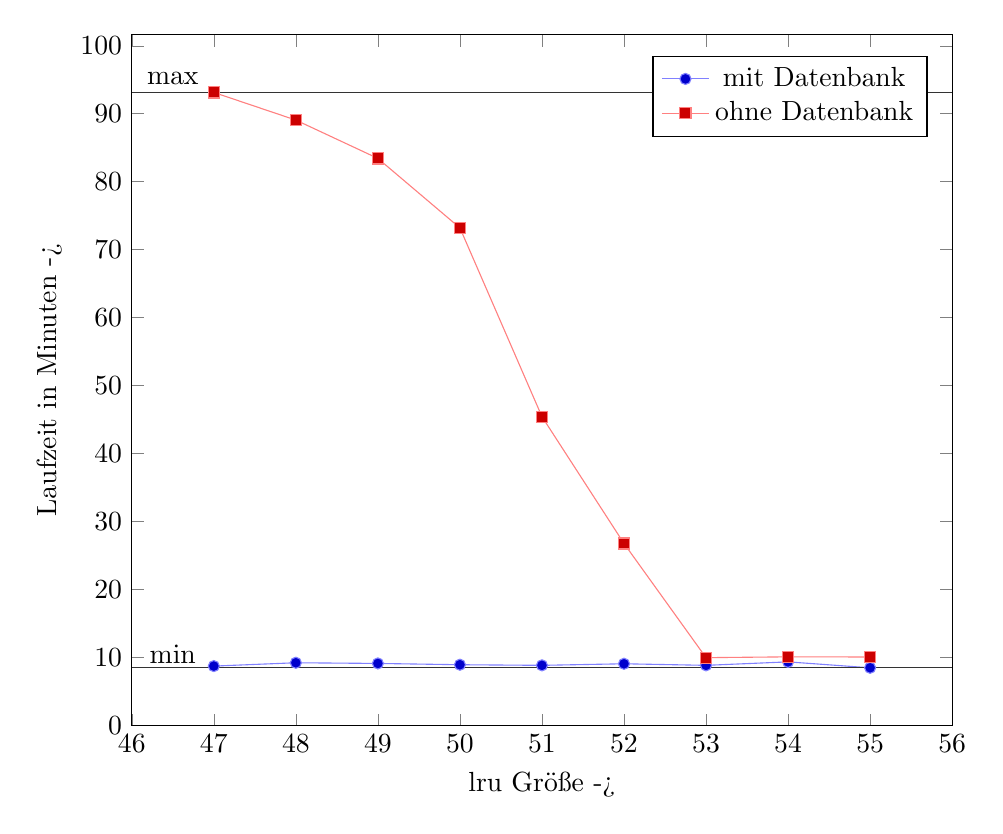
\begin{tikzpicture}
  \begin{axis}[
    width          = 12cm,
    %grid           = both, minor tick num=2,
    %title         = ??,
    xlabel         = \ac{lru} Größe ->,
    ylabel         = Laufzeit in Minuten ->,
    legend pos     = north east,
    ytick distance = 10,
    xmin=46, xmax=56,
    ]

    \tikzstyle{nodetext}=[draw=white, fill=white, draw opacity=0, fill opacity=0, text opacity=1]

    \addplot+[sharp plot, blue!50] coordinates
    {(55, 8.48) (54, 9.35) (53, 8.84) (52, 9.07)
     (51, 8.84) (50, 8.93) (49, 9.12) (48, 9.22) (47, 8.73)};
    \addplot+[sharp plot,  red!50] coordinates
    {(55, 10.07) (54, 10.09) (53, 9.97) (52, 26.77)
     (51, 45.43) (50, 73.20) (49, 83.43) (48, 89.07) (47, 93.14)};

     \addplot[sharp plot,  black!80] coordinates %min
     {(56, 8.48) (46, 8.48)};
     \addplot[sharp plot,  black!80] coordinates %max
     {(56, 93.14) (46, 93.14)};

     \node[nodetext] at (46.5, 10.48) {min};
     \node[nodetext] at (46.5, 95.14) {max};

    \legend{mit Datenbank, ohne Datenbank}
  \end{axis}
\end{tikzpicture}
\caption[Laufzeiten des Systems mit und ohne Datenbank als Cache]{Laufzeiten des Systems (5 Epochs, 53 Datensätze) mit und ohne Datenbank als Cache und variabler \ac{lru} Größe}\label{cap:analyze}
\end{center}
\end{figure}\label{fig:analyze}
